\section{Discretization}

\begin{frame}
\frametitle{Discretizing signals}
Sampling a continuous signal at discrete intervals
\begin{figure}
	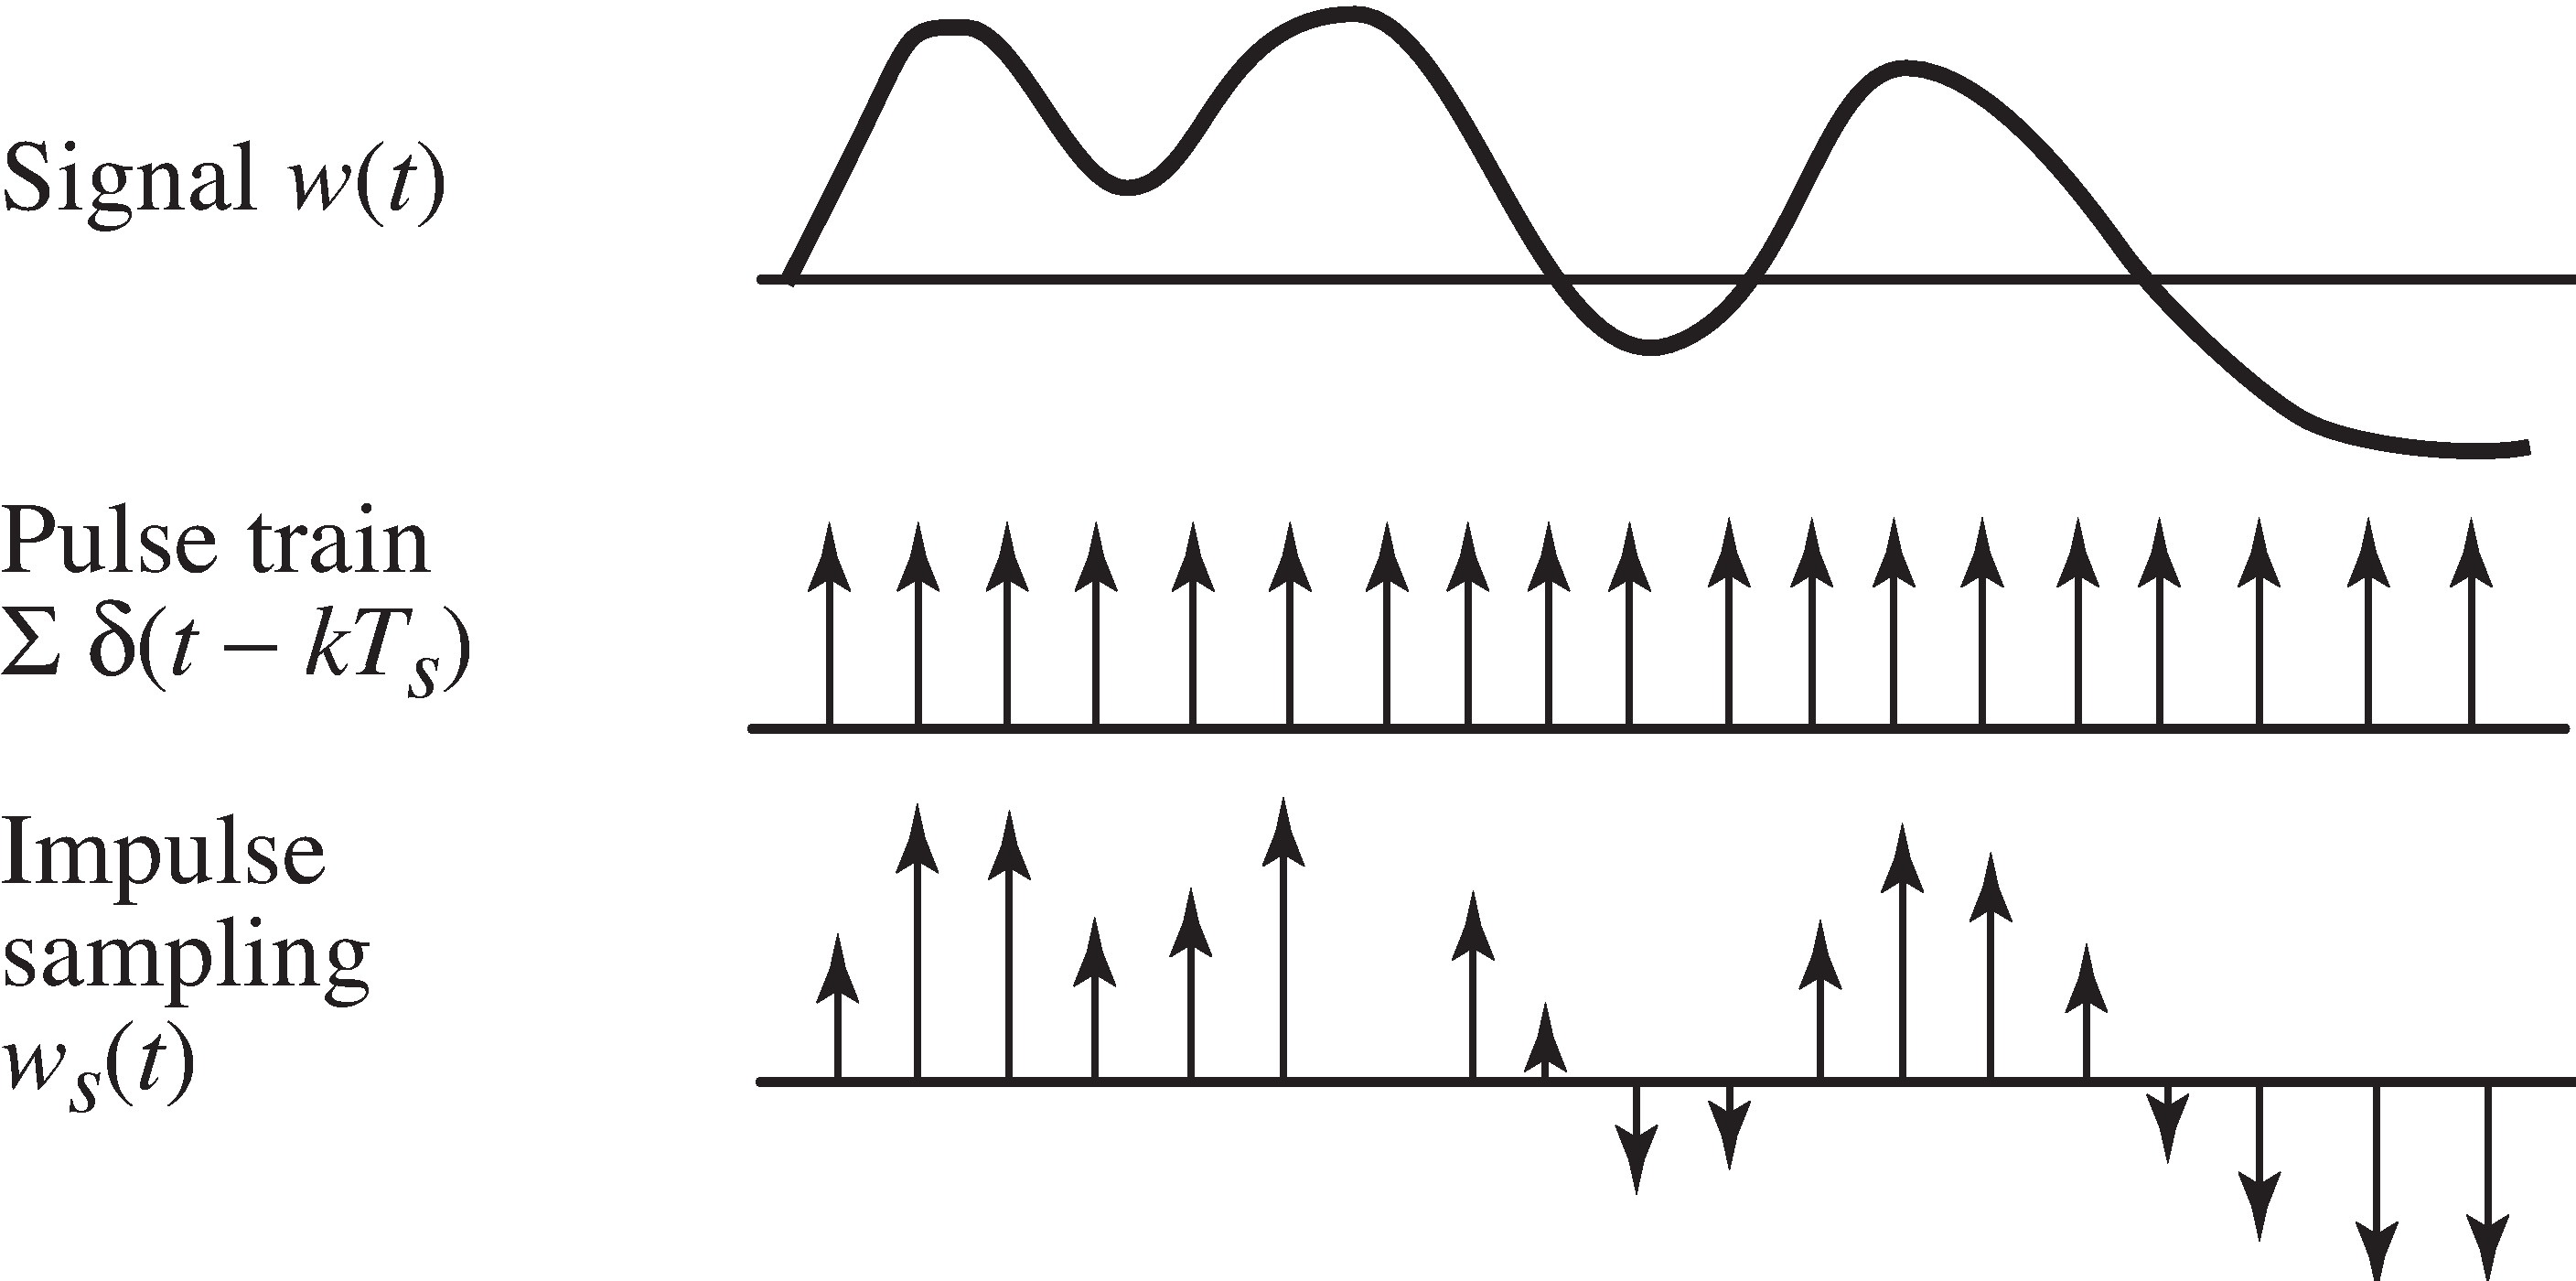
\includegraphics[width=.7\linewidth]{discretization}
\end{figure}
%source: http://cnx.org/contents/42c54126-3078-417f-972e-dcf5c41556a4@3.1:6/Software-Receiver-Design
\end{frame}

\begin{frame}
\frametitle{Discretizing signals}
\vspace{-8ex}
Is it possible to sample a continuous signal without loss of information?\\
\smallskip
Yes, as long as the signal has a limited bandwidth.\\
Bandwidth B = maximum frequency in a signal\\
\bigskip
How often should we sample the signal?\\
\smallskip
Nyquist theorem: if a signal has a bandwidth B then it can be fully reconstructed after being sampled with a frequency 2B
\end{frame}

\subsection{Fourier transform}

\begin{frame}
	\frametitle{Fourier transform}
	\vspace{-2ex}
	\large{\[
	\equalto{f(t)}{\int_{-\infty}^{\infty} e^{j\omega t} d\omega} \Leftrightarrow \equalto{F(j\omega)}{\int_{-\infty}^{\infty} f(\tau) e^{-j \omega \tau} d \tau = |F(j \omega) e^{j \phi(\omega)}|} \in \mathds{C}
	\]}\\
	\begin{figure}
		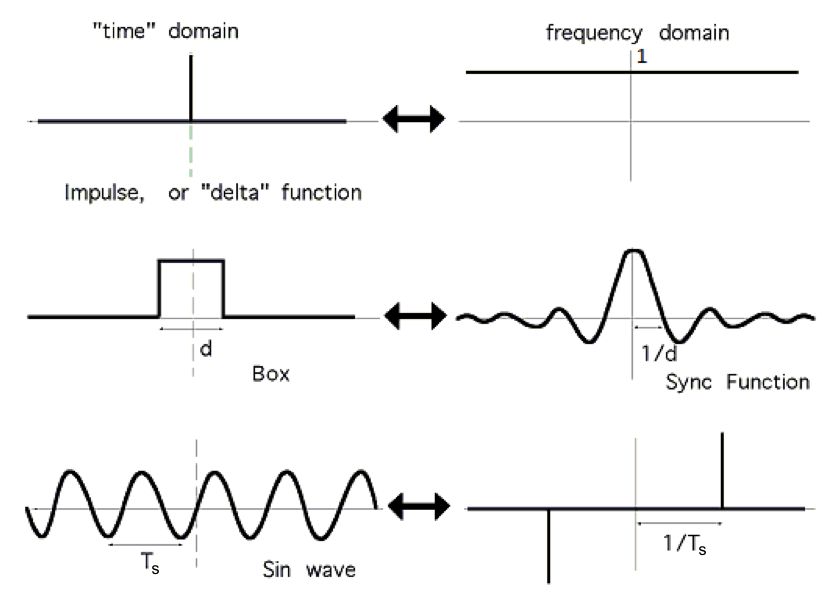
\includegraphics[width=0.6\linewidth]{fourier_examples}
	\end{figure}
\end{frame}

\begin{frame}
	\frametitle{Fourier transform: properties}
	\begin{itemize}
		\item \textbf{Linearity} \\
		\vspace{-3ex}
		\begin{align*}
		& \begin{cases}
		f_1(t) \leftrightarrow F_1(j\omega)\\
		f_2(t) \leftrightarrow F_2(j\omega)
		\end{cases} && \Rightarrow \qquad a f_1(t) + b f_2(t) \leftrightarrow a F_1(j\omega) + b F_2(j \omega)
		\end{align*}
		\item \textbf{Time-scaling} \\
		\medskip
		$f(a t) \leftrightarrow (\frac{1}{|a|}) F(\frac{j \omega}{a})$
		\medskip
		\item \textbf{Translation/Time-shifting} \\
		\medskip
		$f (t - t_0) \leftrightarrow e^{-j \omega t_0} F(j\omega)$
		\medskip
		\item \textbf{Modulation/Frequency-shifting} \\
		\medskip
		$e^{j \omega_0 t} f(t) \leftrightarrow F(j (\omega - \omega_0))$
	\end{itemize}
\end{frame}

\begin{frame}
	\frametitle{Fourier transform: properties}
	\begin{itemize}
		\item \textbf{Reciprocity} \\
		\medskip
		$F(-jt) \leftrightarrow  2 \pi f(\omega)$
		\medskip
		\item \textbf{Derivative in t} \\
		\medskip
		$\frac{df(t)}{dt} \leftrightarrow j\omega F(j\omega) \qquad \qquad \frac{d^nf(t)}{dt^n} \leftrightarrow (j\omega)^n F(j\omega)$
		\medskip
		\item \textbf{Derivative in $\omega$} \\
		\medskip
		$(-jt)^n f(t) \leftrightarrow \frac{d^n F(j\omega)}{d\omega^n} \qquad \frac{f(t)}{-jt} \leftrightarrow \int_{-\infty}^\infty F(j\Omega) d\Omega \> if \> f(0) = 0$
		\medskip
		\item \textbf{Convolution} \\
		\medskip
		$y(t) = h(t) * u(t) \leftrightarrow Y(j\omega) = H(j\omega) U(j\omega)$\\
		$v(t) = h(t)u(t) \leftrightarrow V(j\omega) = \frac{1}{2\pi} H(j\omega)*U(j\omega)$
	\end{itemize}
\end{frame}

\begin{frame}
	\frametitle{Shannon-Nyquist sampling theorem}
	Sampling = multiplication by a train of Dirac-impulses\\
	Fourier transform of an impulse train with period $T$ is an impulse train with period $T^{-1}$:
	\begin{figure}
		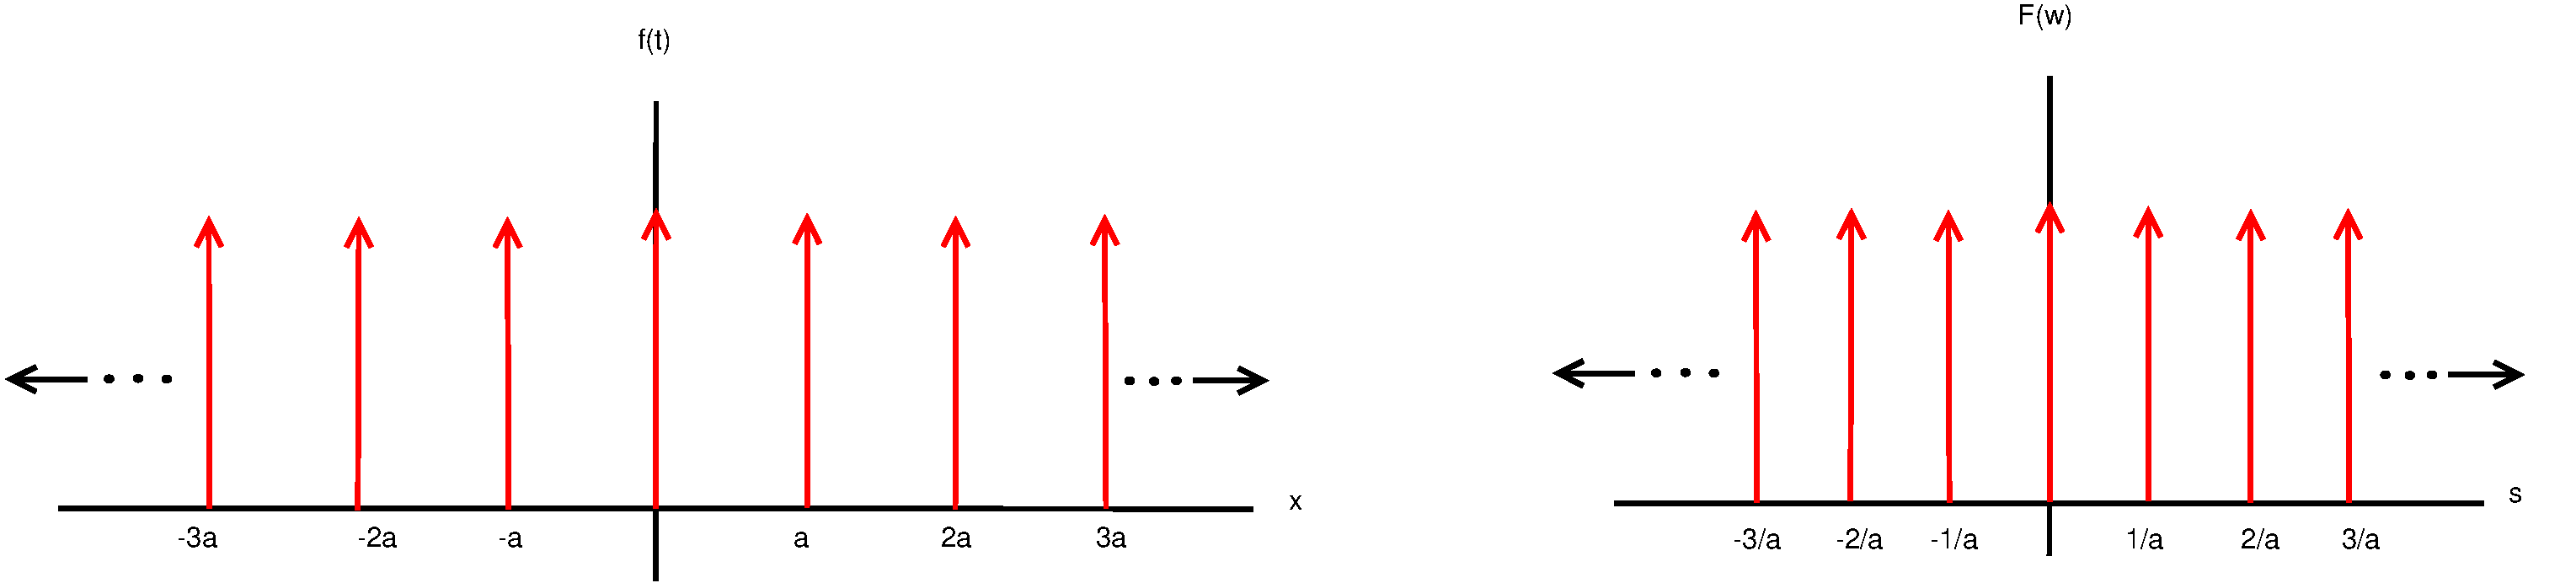
\includegraphics[width=1\linewidth]{fourier_impulse_train}
	\end{figure}
	Sampling in the frequency domain = convolution of signal spectrum and impuls
\end{frame}

\begin{frame}
	\frametitle{Shannon-Nyquist sampling theorem}
	\begin{columns}
		\column{.5\textwidth}
		The signal can be fully reconstructed if there are no overlaps in the frequency domain.\\
		If the sampling frequency is too low then information will be lost (overlap).\\
		If the sampling frequency is at least twice the bandwidth B, then the signal can be reconstructed without a problem (no overlap).\\
		\medskip
		Sampling frequence $f_s \geq 2 B$
		\column{.5\textwidth}
		\begin{figure}
			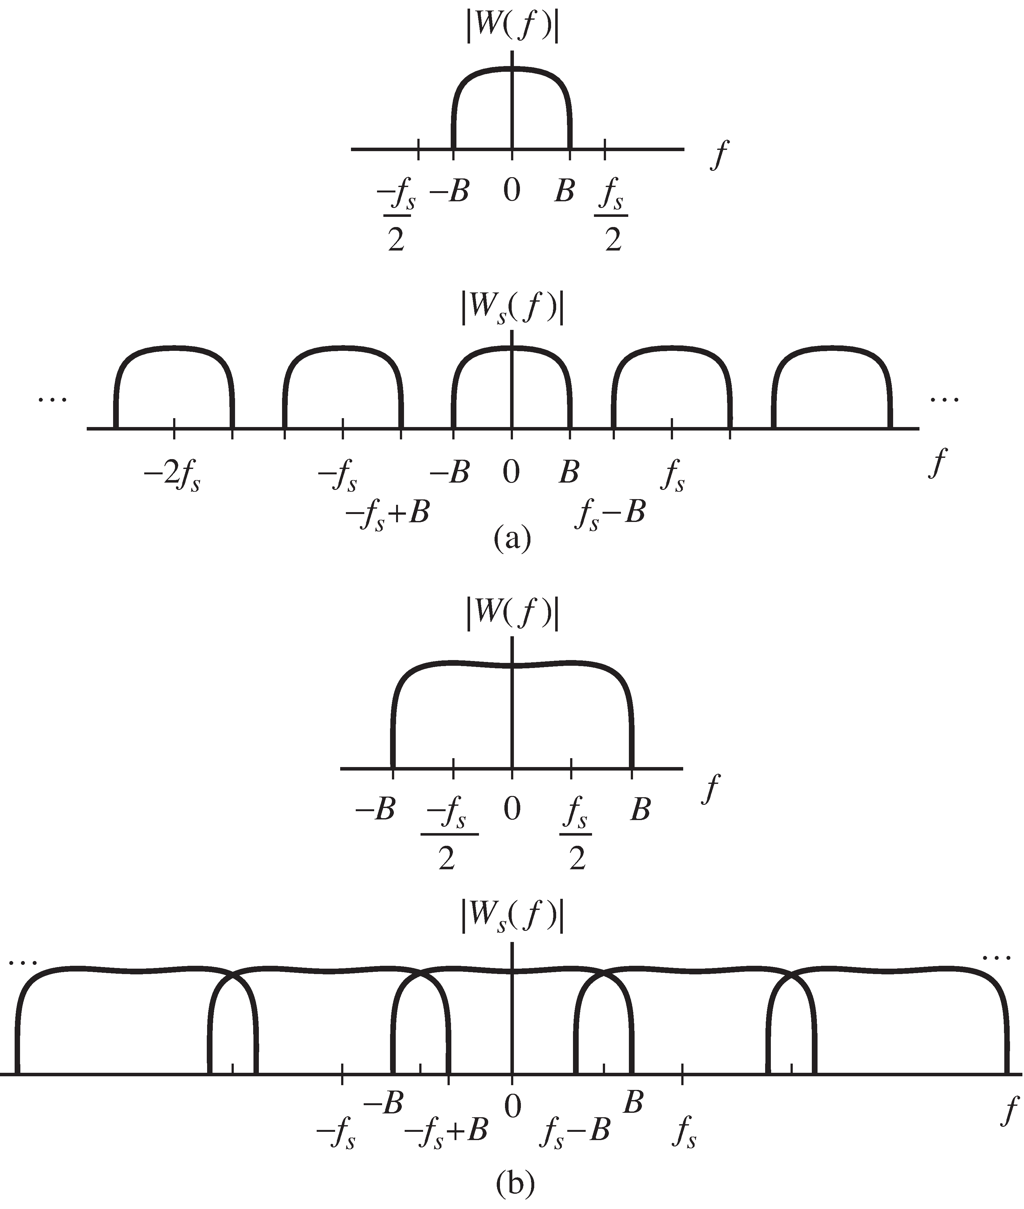
\includegraphics[width=1\linewidth]{nyquist}
		\end{figure}
	\end{columns}
\end{frame}

\subsection{Discretization}

\begin{frame}
	\frametitle{Time sampling}
	\begin{columns}
		\column{.6\textwidth}
		Time sampling is the operation that turns the signal f(t) into a pulse train where the magnitude of the impulse at kT equals the value f(kT).\\
		\medskip
		The choice of the sampling-interval T is important. If T is small enough, the values f(kT) and f((k+1)T) will differ very little. This way we can reconstruct the intermediary values with full accuracy.
		\column{.4\textwidth}
		\begin{figure}
			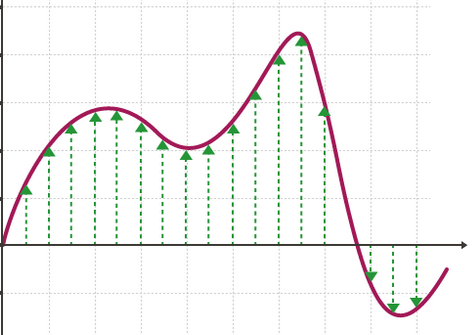
\includegraphics[width=1\linewidth]{signal}
		\end{figure}
	\end{columns}
\end{frame}

\begin{frame}
	\frametitle{Time sampling}
	$y(t) = x(t)c(t) \leftrightarrow Y(f) = \mathcal{F}[y(t)] = \int_{-\infty}^{\infty} y(t)e^{-j2\pi ft} dt$ \\
	$Y(f) = X(f)*C(f)$
	\begin{figure}
		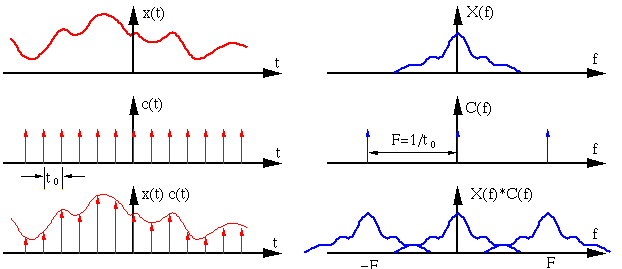
\includegraphics[width=1\linewidth]{time_sampling}
	\end{figure}
\end{frame}

\begin{frame}
	\frametitle{Truncation}
	To get a finite amount of data, we need to truncate the signal by a windowing function of finite duration T, e.g.:\\
	\begin{flalign*}	
	\text{A rectangular window} \\
	&w(t) = 
	\begin{cases}
	1 & 0 \leq t \leq T \\
	0 & otherwise 
	\end{cases}& \\
	\text{with spectrum} \\
	&W(f) = \mathcal{F}[w(t)] = \frac{sin(\pi fT)}{\pi f} e^{-j\pi fT}&
	\end{flalign*}
\end{frame}

\begin{frame}
	\frametitle{Truncation}
	\vspace{-4ex}
	\begin{flalign*} 
	&z(t) = y(t)w(t) = 
	\begin{cases} 
	y(t) & 0 \leq t < T \\ 
	0 & otherwise 
	\end{cases}&\\
	&Z(f) = Y(f)*W(f)&
	\end{flalign*}
	\begin{figure}
		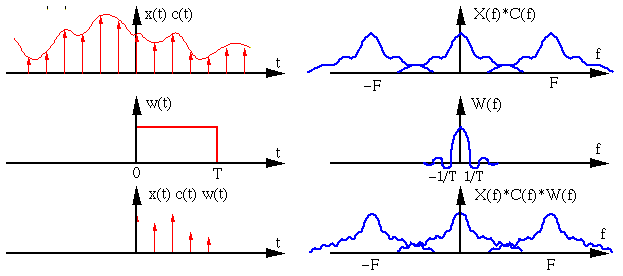
\includegraphics[width=1\linewidth]{truncation}
	\end{figure}
\end{frame}

\begin{frame}
	\frametitle{Frequency sampling}
	\vspace{-4ex}
	\begin{flalign*} 
	&P(j2\pi f) = \sum_{n=-\infty}^{\infty} \delta(f - nf_0) \qquad \leftrightarrow \qquad p(t) = \mathcal{F}^{-1}[P(j2\pi f]&\\
	&V(j2\pi f)= Z(j2\pi f)P(j2\pi f) \qquad \leftrightarrow \qquad v(t) = z(t)p(t) &
	\end{flalign*}
	\begin{figure}
		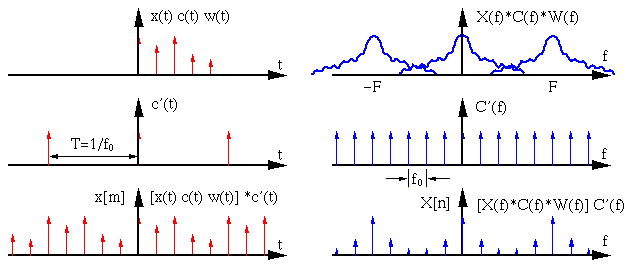
\includegraphics[width=1\linewidth]{frequency_sampling}
	\end{figure}
\end{frame}

\section{Aliasing}

\begin{frame}
	\frametitle{Aliasing}
	Aliasing is	an effect that causes different signals to become indistinguishable when sampled. Frequencies that are too high to be sampled are folded onto lower frequencies.\\
	A too low sample rate doesn't just lose information in the higher frequencies. It also causes faulty values for the lower frequencies.\\
	\vspace{-2ex}
	\begin{figure}
		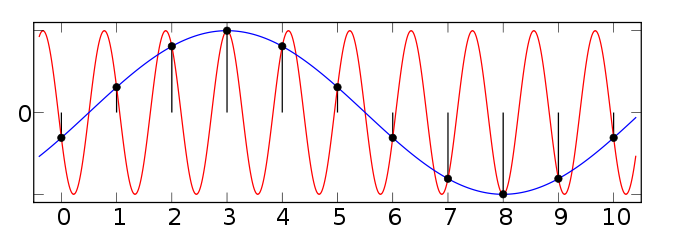
\includegraphics[width=0.7\linewidth]{aliasing}
	\end{figure}
	%source: https://en.wikipedia.org/wiki/Aliasing#/media/File:AliasingSines.svg
	\vspace{-2ex}
	The red sine wave is being sampled at just over it's bandwidth, however the blue sine wave will be recreated as it also fit's all data points and is within the expected bandwidth.
\end{frame}

\section{Reconstruction}

\begin{frame}
	\frametitle{Reconstruction}
	To retrieve the original spectrum of a sampled signal we have to multiply this signal with a block function $H(f) = rect(\frac{t}{t_0})$\\
	\begin{figure}
		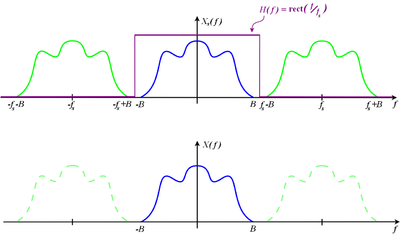
\includegraphics[width=0.6\linewidth]{reconstruct1}
	\end{figure}
	%source: https://upload.wikimedia.org/wikipedia/commons/thumb/1/1f/ReconstructFilter.png/400px-ReconstructFilter.png
	This is the same as convoluting the signal with the inverse Fourier transform of a block function.
\end{frame}

\begin{frame}
	Because convoluting with a shifted impulse shifts a signal, this can be rewritten as:\\
	\medskip
	$\sum_{n=-\infty}^{\infty} f(nT) \frac{sin(\frac{\omega_0(t-nT)}{2})}{\frac{\omega_0(t-nT)}{2}}$\\
	\medskip
	\begin{figure}
		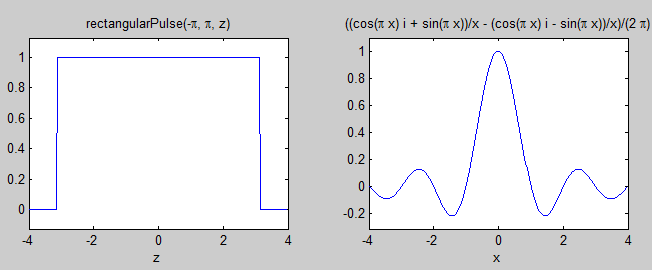
\includegraphics[width=0.8\linewidth]{reconstruct2}
	\end{figure}
\end{frame}

\section{Methods}

\begin{frame}
	\frametitle{Methods}
	Forward Euler\\
	Backward Euler\\
	Trapezium\\
	Bilinear\\
	Prewarping\\
	Zero pole matching\\
	Step invariant (ZOH)\\
	Impuls invariant
\end{frame}

\section{Example}

\begin{frame}
	\frametitle{Title}
	Content
\end{frame}
